\chapter{假设检验}
\section{假设检验的基本思想与概念}
假如试验结果与假设$H$发生矛盾就拒绝原假设H,否则就接受原假设.
\subsection{建设检验问题}
\begin{example}
    女士品茶
\end{example}
\begin{example}
    某厂生产的合金强度服从正态分布$N(\theta,16)$,其中$\theta$ 的设计值为不低千$110 Pa$为保证质量,该厂每天都要对生产情况做例行检查,以判断生产是否正常进行,
    即该合金的平均强度是否不低于$110 Pa$.某天从生产的产品中随机抽取$25$块合金,测得其强度值为$x_{1},x_{2},\cdots,x_{25}.$,均值为$\bar{x}=108.2 Pa$,问当日生产是否正常?
\end{example}


\subsection{假设检验的基本步骤}

\paragraph{一\quad 建立假设} 这里主要叙述参数假设检验问题.设有来自某一个参数分布族$\{F(x,\theta)|\theta \in \Theta\}$的样本$x_1 , x_2 , \cdots,x_n$,其中$\Theta$为参数空间,设$\Theta_0 \subset \Theta$,且$\Theta_0 \neq \varnothing$,则命题$H_0:\theta \in \Theta_0$称为一个假设或\textbf{原假设}或\textbf{零假设},若有另一个$\Theta_1(\Theta_1 \subset \Theta,\Theta_1 \Theta = \varnothing,\text{常见的一种情况是}\Theta_1=\Theta-\Theta_0)$,则命题$H_1:\theta \in \Theta_1$称为$H_0$的\textbf{对立假设}或\textbf{备择假设}.于是,我们感兴趣的一对假设就是
\begin{equation}
    H_0:\theta \in \Theta_0 \quad vs \quad H_1:\theta \in \Theta_1
\end{equation}

如果$\Theta_0$只含一个点,则我们称之为\textbf{简单假设},否则称为\textbf{复杂或复合原假设}.同样,对千备择假设也有简单与复杂之别.当$H_0$为简单假设时,其形式可写成$H_0:\theta=\theta_0$.此时的备择假设通常有如下三种可能:
$$
    H_1^{\prime}:\theta\neq\theta_0,\quad H_1^{\prime\prime}:\theta<\theta_0,\quad H_1^{\prime\prime\prime}:\theta>\theta_0
$$
我们称 $H_{0} \quad vs \quad H$为\textbf{双侧假设}或\textbf{双边假设}(因备择假设分散在原假设两侧而得名),$H_{0} \quad vs \quad H^{\prime\prime}$以及$H_0 \quad vs \quad  H^{\prime\prime\prime}$为\textbf{单侧假设}或\textbf{单边假设}(因备择假设位于原假设的一侧而得名)
在假设检验中,通常将不宜轻易加以否定的假设作为原假设.
\paragraph{二\quad 选择检验统计量,给出拒绝域形式}
当有了具体的样本后,按该法则就可决定是接受$H_0$还是拒绝$H_0$,即检验就等价于把样本空间划分成两个互不相交的部分$W$
和$\overline{W}$,当样本属于$W$时,拒绝$H_0$;否则接受$H_0$。于是,我们称$W$为该检验的\textbf{拒绝域},而$\overline{W}$称为\textbf{接受域}.

由样本对原假设进行检验总是通过一个统计量完成的,该统计量称为\textbf{检验统计量}.比如,在例7.1.2中,样本均值$\overline{x}$就是一个很好的检验统计量,因为要检验的假设是正态总体均值,在方差已知场合,样本均值$\overline{x}$是总体均值的充分统计量。在例7.1.2中,总体均值$\theta$越大,$\overline{x}$取大值大概率越大。亦即,$\overline{x}$越大越支持原假设,$\overline{x}$越小越支持备择假设,所以拒绝域形如
$$
    W=\{(x_{1},x_{2},\cdots,x_{n}):\overline{x}\leq c\}=\{\overline{x}\leq c\}
$$
是合理的,其中临界值$c$待定

当拒绝域确定了,检验的\textbf{判断准则}跟着也确定了:
\begin{itemize}
    \item 如果$(x_1,x_2,\cdots,x_n) \in W$内,则拒绝原假设$H_0$;
    \item 如果$(x_1,x_2,\cdots,x_n) \in \overline{W}$内,则接受原假设$H_0$.
\end{itemize}

\paragraph{三 \quad 选择显著性水平} 两种错误:当$\theta\in\Theta_0$时,样本由于随机性却落入了拒绝域$W$,于是我们采取了拒绝$H_0$的错误决策,称这样的错误为\textbf{第一类错误}(type 1 error);当$\theta \in \Theta_1$,样本却落入接受域$\overline{W}$,于是我们采取了接受$H_0$的错误决策,称这样的错误为\textbf{第二类错误}(type 2 error).
%TODO
在实际中,分别称第一类、第二类错误为拒真错误与取伪错误.

由于检验结果受样本的影响,具有随机性,于是,可用总体分布定义犯第一类、第二类错误概率如下:

犯第一类错误概率:$\alpha(\theta)=P_{\theta}\{X \in W\},\theta \in \Theta_0$

犯第二类错误概率:$\beta(\theta)=P_{\theta}\{X \in \overline{W}\},\theta \in \Theta_1$

\begin{definition}
    设检验问题
    $$
        H_0:\theta\in\Theta_0\quad\mathrm{vs}\quad H_1:\theta\in\Theta_1
    $$
    的拒绝域为$W$,则样本观测值$X$落在拒绝域$W$内的概率称为该检验的\textbf{势函数},记为
    $$
        g(\theta)=P_{\theta}\{X\in W\},\theta\in\Theta=\Theta_0\cup\Theta_1
    $$
\end{definition}
利用这个势函数容易写出其犯两类错误的概率分别为
\begin{equation}
    \begin{aligned}
        \alpha\left(\theta\right) & =\Phi{\left(\frac{c-\theta}{4/5}\right)},\quad\theta\in\Theta_0, \\\beta{\left(\theta\right)}&=1-\Phi{\left(\frac{c-\theta}{4/5}\right)},\quad\theta\in\Theta_1.
    \end{aligned}
\end{equation}
在样本量给定的条件下,$\alpha(\theta)$与$\beta(\theta)$中一个减小必导致另一个增大,这不是偶然的,而具有一般性.这进一步说明:在样本量一定的条件下不可能找到一个使$\alpha(\theta),\beta(\theta)$都小的检验还应注意,犯第二类错误的概率在不少场合不易求出.

通常的做法是仅限制犯第一类错误的概率,这就是费希尔的显著
性检验,下面给出正式定义.
\begin{definition}
    对检验问题$H_0:\theta\in\Theta_0\quad\mathrm{vs}\quad H_1:\theta\in\Theta_1$,如果一个检验满足对任意的$\theta \in \Theta_0 $,都有
    $$
        g(\theta) \le \alpha
    $$
    则称该检验是\textbf{显著性水平}为$\alpha$的\textbf{显著性检验},简称水平为$\alpha$的\textbf{检验}.
\end{definition}

\paragraph{四 \quad 给出拒绝域}
在确定显著性水平后,我们可以定出检验的拒绝域W.在例7.1.2 中,对给定的显著性水平$\alpha$,则要求对任意的$\theta>110$有$g(\theta)=\Phi\left( \frac{5(c-\theta)}{4} \right)\leqslant\alpha $,由于$g(\theta)$是关于$\theta$的单调减函数,只需要
$$g\left(110\right)=\Phi\Big(\frac{5\left(c-110\right)}{4}\Big)=\alpha $$成立即可用标准正态分布分位数可把上式改写为$\frac{5(c-110)}{4}=u_{\alpha}$

若令$u=\frac{\overline{x}-110}{4/5}$,则拒绝域有另一种表示,即$W=\{u\leqslant u_{0.05}\}=\{u\leqslant-1.645\}.$今后主要用检验统计量$u$表示拒绝域.
\paragraph{五 \quad 做出判断}
在有了明确的拒绝域W后,根据样本观测值我们可以作出判断:
\begin{itemize}
    \item 当$\mu \leq -1.645$时,则拒绝$H_0$,即接受$H_1$
    \item 当$\mu > -1.645$时,则接受$H_0$
\end{itemize}
在例7.1.2中,由于
$$u_0=\frac{108.2-110}{4/5}=-2.25<-1.645$$
因此拒绝原假设,即认为该日生产不正常.

综上,一般情况下,寻找某对假设的显著性检验的步骤如下:
\begin{itemize}
    \item 根据实际问题,建立统计假设$H_0 ~v.s.~ H_1 $
    \item 选取一个合适的检验统计量$T(X)$使当凡成立时(或$H_0$中某个具体参数下),$T$的分布完全已知,并根据$H_0$及$H_1$的特点,确定拒绝域$W$的形式.
    \item 选择合适的显著性水平$\alpha$,确定具体的拒绝域$W$.
    \item 由样本观测值$x_1, x_2, \cdots,x_n$,计算检验统计量的$T(x_1,x_2,\cdots,x_n)$,由$T(x_1,x_2,\cdots,x_n)$是否属于$W$,作出最终判断

\end{itemize}

\subsection{检验的p值}
\begin{definition}
    在一个假设检验问题中,利用样本观测值能够作出拒绝原假设的最小显著性水平称为检验的p值.
\end{definition}
也可理解为出现比观测值更极端的样本的概率.

由检验的$p$值与人们心目中的显著性水平$\alpha$进行比较可以很容易作出检验的结论:
\begin{itemize}
    \item 如果$p \leqslant \alpha$,则在显著性水平$\alpha$ 下拒绝$H_0$.
    \item 如果$p > \alpha$,则在显著性水平$\alpha$ 下接受$H_0$.
\end{itemize}
\section{正态总体参数假设检验}
\subsection{单个正态总体均值的假设检验}
设$x_{1},x_{2},\cdots,x_{n}$是来自$ N(\mu,\sigma^{2})$的样本,考虑如下三种关于$\mu$的检验问题:
\begin{align}
    H_0:\mu\leqslant\mu_0\quad vs \quad H_1:\mu>\mu_0 \\
    H_0:\mu\geqslant\mu_0\quad vs \quad H_1:\mu<\mu_0 \\
    H_0:\mu=\mu_0\quad vs \quad H_1:\mu\neq\mu_0
\end{align}

其中$\mu_0$是已知常数由千正态总体含两个参数,总体方差$\sigma^2$已知与否对检验有影响下面我们分$\sigma$已知和未知两种情况叙述.
\paragraph{一、$\sigma=\sigma_0$已知时$\mu$的检验}~{}

对于(7.2.1)式所示的单侧检验间题1,由于$\mu$的点估计是$\bar{x}$,且$\bar{x} \sim  N(\mu,\sigma^2)$故选用检验统计量
\begin{equation}
    u=\frac{\bar{x}-\mu_0}{\sigma_0/\sqrt{n}}
\end{equation}
是恰当的直觉告诉我们:当样本均值$\bar(x)$不超过设定均值$\mu_0$时,应倾向于接受原假设;当样本均值$\bar{x}$超过$\mu_0$时,应倾向于拒绝原假设.可是,在有随机性存在的场合,如果$\bar{x}$比$\mu_0$大一点就拒绝原假设似乎不当,只有当$\bar{x}$比$\mu_0$大到一定程度时拒绝原假设才是恰当的。这就存在一个临界值c,拒绝域为
\begin{equation}
    W_{1}=\{(x_{1},x_{2},\cdots,x_{n}):u\geq c\}
\end{equation}
常简记为$\{u\geq c\}$.若要求检验的显著性水平为$\alpha$,则$c$满足
$$P_{\mu_{0}}(u\geqslant c)=\alpha.$$
由于在$\mu=\mu_0$时,$u\sim N(0,1)$,故$c=u_{1-\alpha}$,,最后的拒绝域为
\begin{equation}
    W_1=\{u\geq u_{1-a}\}
\end{equation}
\begin{figure}[H]
    \centering
    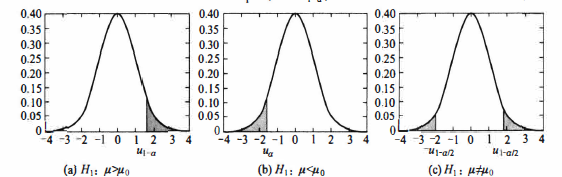
\includegraphics{figures/fig721.png}
\end{figure}
下面我们讲述用p值进行检验的方法.
类似于7.1.3节的讲述,对给定的样本观测值,可以计算出相应的检验统计量$\mu$的值,记$u_{0}=\frac{\sqrt{n}\left(\overline{x}-\mu_{0}\right)}{\sigma_{0}}$这里的$\overline{x}$是样本观测值.因在$\mu=\mu_{0}$时,$u$是服从标准正态分布的随机变量,令
\begin{equation}p_{1}=P(u\geq u_{0})=1-\Phi(u_{0})\end{equation}
此即说明$u_{0}=u_{1-p_{1}}$,于是由正态分布函数的反函数的单调性有如下结论:
\begin{itemize}
    \item 当$p_{1}\leqslant\alpha$时,$u_{1-\alpha}\leq u_{_0}$,于是观测值落在拒绝域里,应拒绝原假设。
    \item 当$p_{1}>\alpha$时,$u_{1-\alpha}>u_{0}$,于是观测值不在拒绝域里,应接受原假设.
\end{itemize}
由此可以看出,上式计算出的值就是该检验的$p$值.

对检验问题(7.2.2)所示的单侧检验问题2的讨论是完全类似的,仍选用$\mu$作为检验统计量,考虑到(7.2.2) 的备择假设$H_1$在左侧,其拒绝域为
\begin{equation}
    W_{2}=\{u\leq u_{_\alpha}\}.
\end{equation}
而检验的p值为
\begin{equation}p_{2}=P(u\leq u_0)=\Phi(u_0),\end{equation}
对检验间题(7.2.3)所示的双侧检验问题3,也可类似进行讨论,只不过检验的$p$值稍有不同仍选用$\mu$作为检验统计量,考虑到(7.2.3)的备择假设几分散在两侧,故其拒绝域亦应在两侧,即拒绝域应有如下形式
$$W_3=\{|u|\geqslant c\}$$
对给定的显著性水平$\alpha (0<\alpha<1)$,由$P_{\mu_{0}}(|u\mid\geq c)=\alpha $可定出$c=\mu_{1-\alpha/2}$最后的拒绝域为
\begin{equation}
    W_3=\{|u|\geqslant \mu_{1-\alpha/2}\}
\end{equation}
下面介绍双侧检验的$p$值的计算.在检验统计量分布对称场合,双侧检验的$p$值的计算与单侧检验是类似的,不对称场合我们在后面介绍.

仿上,令
\begin{equation}P_{3}=P(|u|\geqslant|u_{_0}|)=2(1-\Phi(|u_{_0}|)),\end{equation}
此即说明$|u_{_0}|=\mu_{1-p_{3}/2}$,这里要用到$\mu_0$的绝对值是因为对双侧假设检验,观测值可能为正,也可能为负,二者机会相同,于是有类似的结论:
\begin{itemize}
    \item 当$p_3 \leq \alpha$时,$\mu_{1-\alpha/2} \leq |\mu_0|$,于是观测值落在拒绝域里,应拒绝原假设.
    \item 当$p_3 > \alpha$时,$\mu_{1-\alpha/2} > |\mu_0|$,于是观测值不在拒绝域里,应接受原假设.
\end{itemize}

\paragraph{二、$\sigma$未知时的$t$检验}~{}

对检验问题I,由于$\sigma$ 未知,无法使用(7.2. 4)式作检验.一个自然的想法是将(7.2.4)式中未知的$\sigma$替换成样本标准差$s$,这就形成$t$检验统计量
\begin{equation}
    t = \frac{\sqrt{n}(\bar{x}-\mu_0)}{s}
\end{equation}
由推论5.4.2知,在$\mu=\mu_0$时,$t\sim t(n-1)$,从而检验问题1的拒绝域为
\begin{equation}
    W_1 = \{t \geqslant t_{1-\alpha}(n-1)\}
\end{equation}
检验的$p$值是类似的,对给定的样本观测值,可以计算出相应的检验统计量$t$的值,记为$t_0=\frac{\sqrt{n}(\bar{x}-\mu_0)}{s}$,,这里的$\bar{x},s$可由样本观测值算得.因$t$服从自由度是$n-1$的$t$分布的随机变量,则
\begin{equation}
    p_1 = P(t \geqslant t_0)
\end{equation}
对另两组检验问题的讨论是完全类似于上一小节的,罗列结果如下:检验问题2
的拒绝域为
\begin{equation}
    W_2 = \{t \leqslant t_{\alpha}(n-1)\}
\end{equation}
$p$值为
\begin{equation}
    p_2 = P(t \leqslant t_0)
\end{equation}
检验问题3的拒绝域为
\begin{equation}
    W_3 = \{|t| \geqslant t_{1-\alpha/2}(n-1)\}
\end{equation}
$p$值为
\begin{equation}
    p_3 = P(|t| \geqslant |t_0|)
\end{equation}



\begin{table}[H]
    \caption{单个正态总体均值的假设检验}
    \centering
    \begin{tabular}{cccccc}
        \toprule[1.5pt]
        检验法 & $H_0$            & $H_1$              & 检验统计量 & 拒绝域                               & $p$值                  \\
        \midrule[1pt]
        \multirow{3}{*}{\makecell{$u$检验                                                                                 \\($\sigma = \sigma_0$已知)}} & $\mu \leq \mu_0$  & $\mu > \mu_0$  & \multirow{3}{*}{$u=\frac{\overline{x}-\mu_0}{\sigma_0 / \sqrt{n}}$}  & $\{u \geq u_{1-\alpha}\}$  & $1-\Phi(u_0)$  \\
            & $\mu \geq \mu_0$ & $\mu_1 < \mu_0$    &       & $\{u \leq u_{\alpha}\}$           & $\Phi(u_0)$           \\
            & $\mu = \mu_0$    & $\mu_1 \neq \mu_0$ &       & $\{|u|\geq u_{1-\alpha /2}\}$     & $2(1-\Phi(|u_0|))$    \\
        \addlinespace % 插入一行空白
        \multirow{3}{*}{\makecell{$t$检验                                                                                 \\($\sigma$未知)}} & $\mu \leq \mu_0$ & $\mu > \mu_0$ & \multirow{3}{*}{$t=\frac{\overline{x}-\mu_0}{s /\sqrt{n}}$ }& $\{ t\geq t_{1-\alpha}(n-1)\}$ & $P(t\geqslant t_{0})$\\
            & $\mu \geq \mu_0$ & $\mu < \mu_0$      &       & $\{ t\leq t_{\alpha}(n-1)\}$      & $P(t\leqslant t_{0})$ \\
            & $\mu = \mu_0$    & $\mu \neq \mu_0$   &       & $\{|t|\geq t_{1-\alpha/2}(n-1)\}$ & $P(|t|\geq |t_0|)$    \\
        \bottomrule
    \end{tabular}
\end{table}
注:$u_0=\sqrt{n}(\overline{x}-\mu_0)/\sigma_0,t_0=\sqrt{n}(\overline{x}-\mu_0)/s,u$是服从$N(0,1)$的随机变量,$t$是服从$t(n-1)$的随机变量.

\subsection{假设检验与置信区间的关系}
细心的读者可能会发现,这里用的检验统计昼与6.6.3节中置信区间所用的枢轴
量很相似,这不是偶然的,两者之间存在非常密切的关系,现以标准差未知场合为例叙述如下.
设$x_{1},x_{2},\cdots,x_{n}$是来自正态总体$N(\mu,\sigma^2)$的样本,现讨论在$\sigma$未知场合关于均值$\mu$的检验问题.分三种情况:

首先考虑双侧检验问题3,显著性水平为$\alpha$的检验的接受域为
$$\overline{W}_3=\{| \overline{x}-\mu_{0}| \leq\frac{s}{\sqrt{n}}t_{1-\alpha/2}(n-1)\}$$
它可以改写为
$$
    \bar{W} = \{ \bar{x}-\frac{s}{\sqrt{n}}t_{1-\alpha/2}(n-1) \leq \mu_0 \leq \bar{x} +\frac{s}{\sqrt{n}}t_{1-\alpha/2}(n-1) \}
$$
这里$\mu$并无限制,若让$\mu_0$在$(-\infty,\infty)$内取值,就可得到$\mu$的$1-\alpha$置信区间$\left[\overline{x}\pm\frac{s}{\sqrt{n}}t_{1-a/2}(n-1)\right]$。反之,若有一个如上的$1-\alpha$置信区间,也可获得关于$H_0:\mu=\mu_0$的显著性水平为$\alpha$的显著性检验。所以,“正态均值$\mu$的$1-\alpha$置信区间”与“ 关于$H_0:\mu=\mu_0 \quad vs \quad H_1:\mu \neq \mu_0$的双侧检验问题的显著性水平为$\alpha$的检验”是一一对应的。

类似地考虑单侧检验问题I,显著性水平为$\alpha$的检验的接受域为
$$\overline{W}_{1}=\left\{\overline{x}-\mu_{0}\leqslant\frac{s}{\sqrt{n}}t_{1-\alpha}(n-1)\right\}=\left\{\mu_{0}\geqslant\overline{x}-\frac{s}{\sqrt{n}}t_{1-\alpha}(n-1)\right\}$$这就给出了参数$\mu$的$1-\alpha$置信下限.反之,对上述给定的$\mu$的$1-\alpha$置信下限,我们也可以得到关于$H_0:\mu\leq \mu_0$的单侧检验问题的显著性水平为$\alpha$的检验,它们之间也是一一
对应的同样,对单侧检验问题2,其显著性水平为$\alpha$的检验与参数$\mu$的$1-\alpha$置信上限也是一一对应的.
\subsection{两个正态总体均值差的假设检验}
设$x_{1},x_{2},\cdots,x_{m}$是来自正态总体$N(\mu_1,\sigma_1^2)$的样本,$y_{1},y_{2},\cdots,y_{n}$是来自另一个正态总体$N(\mu_2,\sigma_2^2)$的样本,两个样本相互独立考虑如下三类检验问题:
\begin{align}
    H_{0}:\mu_{1}-\mu_{2} \leq 0 \quad vs \quad H_{1}:\mu_{1}-\mu_{2}>0.      \\
    H_{0}:\mu_{1}-\mu_{2}\geqslant 0  \quad vs \quad H_{1}:\mu_{1}-\mu_{2}<0. \\
    H_{0}:\mu_{1}-\mu_{2}=0 \quad vs \quad H_{1}:\mu_{1}-\mu_{2}\neq0.
\end{align}
\paragraph{一、$\sigma_1,\sigma_2$已知时两样本$\mu$的检验}~{}

此时$\mu_1-\mu_2$的点估计$\bar{x}-\bar{y}$的分布完全已知,
$$\overline{x}-\overline{y}-N\left(\mu,-\mu_{2},\frac{\sigma_{1}^{2}}{m}+\frac{\sigma_{2}^{2}}{n}\right).$$
由此可采用u检验方法,检验统计量为
$$u=\frac{\overline{x}-\overline{y}}{\sqrt{\frac{\sigma_{1}^{2}}{m}+\frac{\sigma_{2}^{2}}{n}}}.$$
在$\mu_1=\mu_2$时,$\mu\sim N(0,1)$。检验的拒绝域取决于备择假设的具体内容.对(7.2.19)所示的检验问题1,检验的拒绝域与$p$值分别为
$$W_{1}=\{ u\geq u_{1-\alpha}\},\quad p_{1}=1-\Phi(u_{0})$$
其中$u_{0}=\frac{\overline{x}-\overline{y}}{\sqrt{\frac{\sigma_{1}^{2}}{m}+\frac{\sigma_{2}^{2}}{n}}}$是由样本计算得到的检验统计量的值.对(7.2.20)所示的检验问题2,检验的拒绝域与$p$值分别为
$$W_{2}=\{ u\leq u_{\alpha}\},\quad p_{2}=\Phi(u_{0})$$
对(7.2.21)所示的检验问题3,检验的拒绝域与$p$值分别为
$$W_{3}=\{ |u|\geq u_{1-\alpha/2}\},\quad p_{3}=2(1-\Phi(|u_{0}|))$$

\paragraph{二、$\sigma_1=\sigma_2=\sigma$但未知的两样本$t$检验}~{}

在$\sigma_1=\sigma_2=\sigma$但未知时,首先
$$\bar{x}-\bar{y}\sim N\left(\left.\mu_1-\mu_{2},\left(\frac{1}{m}+\frac{1}{n}\right)\sigma^{2}\right.\right)$$
其次,由于
$$\frac1{\sigma^2}\sum_{i=1}^m{(x_i-\overline{x})^2}\quad\sim{\mathcal X}^2(m-1),\quad\frac1{\sigma^2}\sum_{i=1}^n{(y_i-\overline{y})^2}\quad\sim{\mathcal X}^2(n-1)$$
故$\frac{1}{\sigma^{2}}(\sum(x_{i}-\overline{x})^{2}+\sum(y_{i}-\overline{y})^{2})-\chi^{2}(m+n-2)$,记
$$s_{w}^{2}=\frac{1}{m+n-2}\Big[\sum_{i=1}^{m}(x_{i}-\overline{x})^{2}+\sum_{i=1}^{n}(y_{i}-\overline{y})^{2}\Big]$$
于是有
$$t=\frac{(\overline{x}-\overline{y})-(\mu_{1}-\mu_{2})}{s_{w}\sqrt{\frac{1}{m}+\frac{1}{n}}}\sim t(m+n-2)$$
当$\mu_1=\mu_2$时,检验统计量为
$$t=\frac{\overline{x}-\overline{y}}{s_{_w}\sqrt{\frac1m+\frac1n}}$$
对检验问题1,检验的拒绝域与$p$值分别为
$$W_{1}= \{ t\geqslant t_{1-\alpha}(m+n-2)\},\quad p_{1}=P(t\geqslant t_{0})$$
其中$t_0=\frac{\overline{x}-\overline{y}}{s_{_w}\sqrt{\frac1m+\frac1n}}$是由样本计算得到的检验统计量的值,$t$是服从自由度是$n+m-2$的$t$分布的随机变量.对检验问题2,检验的拒绝域与$p$值分别为
$$W_{2}=\{ t\leq t_{\alpha}(m+n-2)\},\quad p_{2}=P(t\leq t_{0}).$$
对检验问题3,检验的拒绝域与$p$值分别为
$$W_{3}=\{ |t|\geq t_{1-\alpha/2}(m+n-2)\},\quad p_{3}=P(|t|\geq |t_{0}|).$$


\begin{table}[H]
    \caption{两个正态总体均值的假设检验}
    \centering
    \begin{tabular}{cccccc}
        \toprule[1.5pt]
        检验法 & $H_0$              & $H_1$              & 检验统计量 & 拒绝域                                 & $p$值                      \\
        \midrule[1pt]
        \multirow{3}{*}{\makecell{$u$检验                                                                                         \\($\sigma_1,\sigma_2$已知)}} & $\mu_1 \leq \mu_2$  & $\mu_1 > \mu_2$  & \multirow{3}{*}{$u=\frac{\overline{x}-\overline{y}}{\sqrt{\frac{\sigma_{_1}^2}m+\frac{\sigma_{_2}^2}n}}$}  & $\{u \geq u_{1-\alpha}\}$  & $1-\Phi(u_1)$  \\
            & $\mu_1 \geq \mu_2$ & $\mu_1 < \mu_2$    &       & $\{u \leq u_{\alpha}\}$             & $\Phi(u_1)$               \\
            & $\mu_1 = \mu_2$    & $\mu_1 \neq \mu_2$ &       & $\{|u|\geq u_{1-\alpha /2}\}$       & $2(1-\Phi(|u_1|))$        \\
        \addlinespace % 插入一行空白
        \multirow{3}{*}{\makecell{$t$检验                                                                                         \\($\sigma_1=\sigma_2$未知)}} & $\mu_1 \leq \mu_2$ & $\mu_1 > \mu_2$ & \multirow{3}{*}{$t=\frac{\overline{x}-\overline{y}}{s_{w}\sqrt{\frac1m+\frac1n}}$ }& $\{ t\geq t_{1-\alpha}(m+n-2)\}$ & $P(T_{1}\geqslant t_{1})$\\
            & $\mu_1 \geq \mu_2$ & $\mu_1 < \mu_2$    &       & $\{ t\leq t_{\alpha}(m+n-2)\}$      & $P(T_{1}\leqslant t_{1})$ \\
            & $\mu_1 = \mu_2$    & $\mu_1 \neq \mu_2$ &       & $\{|t|\geq t_{1-\alpha/2}(m+n-2)\}$ & $P(|T_1|\geq |t_1|)$      \\
        \bottomrule
    \end{tabular}
\end{table}

\begin{table}[H]
    \caption{两个正态总体均值的假设检验\label{tab:experiment1}}
    \centering
    \begin{tabular}{cccccc}
        \toprule[1.5pt]
        检验法 & $H_0$              & $H_1$              & 检验统计量 & 拒绝域                             & $p$值                      \\
        \midrule[1pt]
        \multirow{3}{*}{\makecell{大样本$u$检验                                                                                  \\($m,n$充分大)}} & $\mu_1 \leq \mu_2$  & $\mu_1 > \mu_2$  & \multirow{3}{*}{$u=\frac{\overline{x}-\overline{y}}{\sqrt{\frac{s_x^2}m+\frac{s_y^2}n}}$}  & $\{u \geq u_{1-\alpha}\}$  & $1-\Phi(u_2)$  \\
            & $\mu_1 \geq \mu_2$ & $\mu_1 < \mu_2$    &       & $\{u \leq u_{\alpha}\}$         & $\Phi(u_2)$               \\
            & $\mu_1 = \mu_2$    & $\mu_1 \neq \mu_2$ &       & $\{|u|\geq u_{1-\alpha /2}\}$   & $2(1-\Phi(|u_2|))$        \\
        \addlinespace % 插入一行空白
        \multirow{3}{*}{\makecell{近似$t$检验                                                                                   \\($m,n$不很大)}} & $\mu_1 \leq \mu_2$ & $\mu_1 > \mu_2$ & \multirow{3}{*}{$t=\frac{\overline{x}-\overline{y}}{\sqrt{\frac{s_x^2}{m}+\frac{x_y^2}{n}  }}$ }& $\{ t\geq t_{1-\alpha}(l)\}$ & $P(T_{1}\geqslant t_{2})$\\
            & $\mu_1 \geq \mu_2$ & $\mu_1 < \mu_2$    &       & $\{ t\leq t_{\alpha}(l)\}$      & $P(T_{1}\leqslant t_{2})$ \\
            & $\mu_1 = \mu_2$    & $\mu_1 \neq \mu_2$ &       & $\{|t|\geq t_{1-\alpha/2}(l)\}$ & $P(|T_1|\geq |t_2|)$      \\
        \bottomrule
    \end{tabular}
\end{table}
注:$u_{1}=\frac{\overline{x}-\overline{y}}{\sqrt{\frac{\sigma_{1}^{2}}{m}+\frac{\sigma_{2}^{2}}{n}}}$,$u_{2}=\frac{\overline{x}-\overline{y}}{\sqrt{\frac{s_{x}^{2}}{m}+\frac{s_{y}^{2}}{n}}}$,$t_{1}=\frac{\overline{x}-\overline{y}}{s_{w}\sqrt{\frac{1}{m}+\frac{1}{n}}}$,$t_{2}=\frac{\overline{x}-\overline{y}}{\sqrt{\frac{s_{x}^{2}}{m}+\frac{s_{y}^{2}}{n}}}$,$T_1$是服从自由度为$n+m-2$的$t$分布的随机变量, $T_2$是服从自由度为$l$的$t$分布的随机变量, $l$与$s_w$的表达式见6.6.6 节
\subsection{成对数据检验}
在对两个总体均值进行比较时, 有时数据是成对出现的,此时若采用二样本t检验所得出的结论有可能是不对的,下面看一个例子.
\subsection{正态总体方差的检验}
\paragraph{一、单个正态总体方差的$\chi^2$检验}~{}
设$x_{1},x_{2},\cdots,x_{m}$是来自正态总体$N(\mu,\sigma^2)$的样本,对方差亦可考虑如下三个检验问题:
\begin{align}
    H_{0}:\sigma^{2}\leq\sigma_{0}^{2} \quad vs \quad H_{1}:\sigma^{2}>\sigma_{0}^{2}. \\
    H_{0}:\sigma^{2}\geq\sigma_{0}^{2} \quad vs \quad H_{1}:\sigma^{2}<\sigma_{0}^{2}. \\
    H_{0}:\sigma^{2}=\sigma_{0}^{2} \quad vs \quad H_{1}:\sigma^{2}\neq\sigma_{0}^{2}.
\end{align}
其中$\sigma_0$是已知常数。此处通常假定$\mu$未知,它们采用的检验统计量是相同的,均为
\begin{equation}\mathcal {X}^{2}=\left({n-1}\\ \right)s^{2}/\sigma_{0}^{2}.\end{equation}
在$\sigma^2=\sigma_0^2$时,$\chi^2\sim \chi^2(n-1)$,于是,若取显著性水平为$\alpha$,则对应三个检验间题的显著性水平为$\alpha$的检验的拒绝域依次为
$$
    \begin{aligned}
        W_{1} & =\{\chi^{2}\geq\chi_{1-\alpha}^{2}(n-1)\},                                                           \\
        W_{2} & =\{\chi^{2}\leq\chi_{\alpha}^{2}(n-1)\},                                                             \\
        W_{3} & =\{\chi^{2}\leq\chi_{\alpha/2}^{2}(n-1)\quad\text{or}\quad\chi^{2} \geq \chi_{1-\alpha/2}^{2}(n-1)\}
    \end{aligned}
$$

我们亦可给出检验的$p$值.对单侧检验,想法是类似的,记 ${\mathcal X}_{0}^{2}=(n-1)s^{2}/\sigma_{0}^{2}$是由样本计算得到的检验统计量的值,$\chi^2$表示服从自由度为$n-1$的$\chi^2$分布的随机变量,则检
验问题1, 2的$p$值分别为$p_1=P(\chi^2 \geq \chi_0^2)$,$p_2 = P(\chi^2 \leq \chi_0^2)$。对双侧检验则稍稍复杂一
点,事实上,双侧检验的拒绝域在两侧,用$\chi_0^2$可算得两个尾概率$P(\chi^2 \leq \chi_0^2)$和$P(\chi^2 \geq \chi_0^2)$,其和为1 ,其中必有一个$\leq 0.5$.检验的注意力总放在拒绝域上,故应从中选一个小
的与$\alpha / 2$比较,从而检验问题3的$p$值为
\begin{equation}
    p_3 = 2\min\{P(\chi^2 \leq \chi_0^2),P(\chi^2 \geq \chi_0^2)\}
\end{equation}
对这样定义的p值,不难发现下述结论仍然是成立的:


\begin{itemize}
    \item 当$p_3 \leq \alpha$时,应拒绝原假设
    \item 当$p_3 > \alpha$时,应接受原假设
\end{itemize}

\paragraph{二、两个正态总体方差比的$F$检验}~{}

设$x_{1},x_{2},\cdots,x_{m}$是来自$N(\mu_1,\sigma_1^2)$的样本,$y_{1},y_{2},\cdots,y_{n}$是来自$N(\mu_2,\sigma_2^2)$的样本,考虑如下三个假设检验问题:
\begin{align}
    H_{0}:\sigma_{1}^{2} \leq \sigma_{2}^{2} \quad vs \quad H_{1}:\sigma_{1}^{2}>\sigma_{2}^{2}. \\
    H_{0}:\sigma_{1}^{2} \geq \sigma_{2}^{2} \quad vs \quad H_{1}:\sigma_{1}^{2}<\sigma_{2}^{2}. \\
    H_{0}:\sigma_{1}^{2}=\sigma_{2}^{2} \quad vs \quad H_{1}:\sigma_{1}^{2}\neq\sigma_{2}^{2}.
\end{align}
此处$\mu_1,\mu_2$均未知,记$s_x^2,s_y^2$分别是由$x_1,x_2,\cdots,x_m$算得的$\sigma^1$的无偏估计和由$y_1,y_2,\cdots,y_n$算得的$\sigma^2$的无偏估计,即(两个都是样本方差),则可建立如下的检验统计量:
\begin{equation}
    F = \frac{s_x^2}{s_y^2}
\end{equation}
当$\sigma_1=\sigma_2$时,$F\sim F(m-1,n-1)$,由此给出三个检验问题对应的拒绝域依次为:
$$
    \begin{aligned}
        W_{1} & =\{F\geq F_{1-\alpha}(m-1,n-1)\},                                                 \\
        W_{2} & =\{F\leq F_{\alpha}(m-1,n-1)\},                                                   \\
        W_{3} & =\{F\leq F_{\alpha/2}(m-1,n-1)\quad\text{or}\quad F\geq F_{1-\alpha/2}(m-1,n-1)\}
    \end{aligned}
$$
此时检验的$p$值的讨论与前述$\chi^2$是相似的,记$F_0=s_x^2/s_y^2$,是由样本计算得到的检验统计量的值,$F$表示服从$F(m-1,n-1)$分布的随机变量,则检验问题1,2,3的$p$值分别为
$$
    \begin{aligned}
        p_1 & =P(F\geq F_0),                      \\
        p_2 & =P(F\leq F_0),                      \\
        p_3 & =2\min\{P(F\geq F_0),P(F\leq F_0)\}
    \end{aligned}
$$

\begin{table}[H]
    \caption{正态总体方差的假设检验}
    \centering
    \begin{tabular}{cccccc}
        \toprule[1.5pt]
        检验法                         & $H_0$                        & $H_1$                        & 检验统计量                                                   & 拒绝域                                              & $p$值                      \\
        \midrule[1pt]
        \multirow{3}{*}{$\chi^2$检验} & $\sigma^2 \leq \sigma_0^2$   & $\sigma^2 > \sigma_0^2$      & \multirow{3}{*}{$\chi^2=\frac{(n - 1)s^2}{\sigma_0^2}$} & $\chi^2 \geq \chi_{1-\alpha}^2(n-1)$             & $P(\chi^2 \geq \chi_0^2)$ \\

                                    & $\sigma^2 \geq \sigma_0^2$   & $\sigma^2 < \sigma_0^2$      &                                                         & $\chi^2 \leq \chi_{\alpha}^2(n-1)$               & $P(\chi^2 \leq \chi^2_0)$ \\

                                    & $\sigma^2 = \sigma_0^2$      & $\sigma^2 \neq \sigma_0^2$   &                                                         & \makecell{$\chi^2 \leq \chi_{\alpha /2}^2(n-1)$或                             \\$\chi^2 \geq \chi_{1-\alpha /2}^2(n-1) $} &\makecell{$2\min\{P(\chi^{2}\leq \chi_{0}^{2}),$\\$P(\chi^{2}\geq \chi_{0}^{2})\}$}\\
        \midrule
        \multirow{3}{*}{$F$检验}      & $\sigma_1^2 \leq \sigma_2^2$ & $\sigma_1^2 > \sigma_2^2$    & \multirow{3}{*}{$F=\frac{s_x^2}{s_y^2}$}                & $F \geq F_{1-\alpha}(m-1,n-1)$                   & $P(F \geq F_0)$           \\

                                    & $\sigma_1^2 \geq \sigma_2^2$ & $\sigma_1^2 < \sigma_2^2$    &                                                         & $F \leq F_{\alpha}(m-1,n-1)$                     & $P(F \leq F_0)$           \\

                                    & $\sigma_1^2 = \sigma_2^2$    & $\sigma_1^2 \neq \sigma_2^2$ &                                                         & \makecell{$F\leq F_{\alpha/2}(m-1,n-1)$或                                     \\$F \geq F_{1-\alpha/2}(m-1,n-1)$} &\makecell{$2\min\{P(F\leq F_0),$\\ $P(F \geq F_0)\}$} \\
        \bottomrule
    \end{tabular}
\end{table}
\section{其他分布参数的假设检验}
\subsection{指数分布参数的假设检验}
指数分布是一类重要的分布,有广泛的应用.设$x_1,x_2,\cdots,x_n$是来自指数分布$Exp(1/\theta)$的样本,$\theta$为其均值,现考虑关于$\theta$的如下检验问题:
\begin{equation}
    H_0:\theta \leq \theta_0 \quad vs \quad H_1:\theta > \theta_0
\end{equation}
为寻找检验统计量, 我们考察参数$\theta$的充分统计量$\bar{x}$,在$\theta=\theta_0$时,$n \bar{x}=\sum_{i=1}^nx_i\sim Ga(n,1/\theta_0)$,由伽马分布性质可知
\begin{equation}
    \chi^2=\frac{2n\bar{x}}{\theta_0}\sim \chi^2(2n)
\end{equation}
于是可用$\chi^2$作为检验统计量并利用$\chi^2(2n)$的分位数建立检验的拒绝域,对检验问题(7.3. l),拒绝域形式为$W_1=\{\chi^2 \geq c\}$,对给定的显著性水平$\alpha$,可由$P(W_1)=\alpha$获得拒绝域如下:
\begin{equation}
    W_1=\{\chi^2 \geq \chi_{1-\alpha}^2(2n)\}
\end{equation}
类似本章前面关于检验的$p$值的讨论,记${\mathcal X}_{0}^{2}=\frac{2n\overline{x}}{\theta_{0}}$为由样本算得的检验统计量值,$\chi^2$表示服从$\chi^2(2n)$分布的随机变量,则检验的$p$值为$p_1=P(\chi^2 \geq \chi_0^2)$

关于0的另两种检验间题处理方法类似.对检验问题
$$
    2\quad H_0:\theta \geq \theta_0 \quad vs \quad H_1:\theta < \theta_0 \quad \text{and} \quad 3 \quad H_0:\theta = \theta_0 \quad vs \quad H_1:\theta \neq \theta_0
$$
检验统计量不变,拒绝域以及检验的$p$值分别为
$$
    \begin{aligned}
        W_2 & = \{\chi^2 \leq \chi_{\alpha}^2(2n)\}, \quad p_2 = P(\chi^2 \leq \chi_0^2)                                                                                              \\
        W_3 & = \{\chi^2 \leq \chi_{\alpha/2}^2(2n) \quad \text{or} \quad \chi^2 \geq \chi_{1-\alpha/2}^2(2n)\}, \quad p_3 = 2\min\{P(\chi^2 \geq \chi_0^2),P(\chi^2 \leq \chi_0^2)\}
    \end{aligned}
$$

\begin{table}[H]
    \caption{指数分布均值$\theta$的假设检验}
    \centering
    \begin{tabular}{cccccc}
        \toprule[1.5pt]
        检验法                         & $H_0$                        & $H_1$                        & 检验统计量                                                   & 拒绝域                                              & $p$值                      \\
        \midrule[1pt]
        \multirow{3}{*}{$\chi^2$检验} & $\theta \leq \theta_0$   & $\theta > \theta_0$      & \multirow{3}{*}{$\chi^2=\frac{2n \overline{x}}{\theta_0}$} & $\chi^2 \geq \chi_{1-\alpha}^2(2n)$             & $P(\chi^2 \geq \chi_0^2)$ \\

        & $\theta \geq \theta_0$   & $\theta< \theta_0$      &                                                         & $\chi^2 \leq \chi_{\alpha}^2(2n)$               & $P(\chi^2 \leq \chi^2_0)$ \\

        & $\theta= \theta_0$      & $\theta \neq \theta_0$   &                                                         & \makecell{$\chi^2 \leq \chi_{\alpha /2}^2(2n)$或 \\
        $\chi^2 \geq \chi_{1-\alpha /2}^2(2n) $} &\makecell{$2\min\{P(\chi^{2}\leq \chi_{0}^{2}),$\\$P(\chi^{2}\geq \chi_{0}^{2})\}$}\\
        \bottomrule
    \end{tabular}
\end{table}
\subsection{比率p的检验}
比率$p$可看作某事件发生的概率,即可看作二点分布$b(1,p)$中的参数,作$n$次独立试验,以$x$记该事件发生的次数,则$x \sim b(n,p)$。我们可以根据$x$检验关于$p$的一些假设。考虑如下单边假设检验问题:
\begin{equation}
    1 \quad H_0:p \leq p_0 \quad vs \quad H_1:p > p_0
\end{equation}
直观上看,一个显然的检验方法是取如下的拒绝域$W=\{x\geq c\}$,由于$x$只取整数值,故$c$可限制在非负整数中然而,一般情况下对给定的$\alpha$,不一定能正好取到一个c,使得
\begin{equation}
    P(x \geq c;p_{_0}) = \sum_{i=c}^{n}\tbinom{n}{i}p_{_0}^i(1-p_{_0})^{n-i} = \alpha
\end{equation}
能恰巧使得(7.3 .5)成立的$c$值是罕见的.这是在对离散总体作假设检验中普遍会遇到的问题,在这种情况下,较常见的是找一个$C_0$,使得
$$\sum_{i=c_0}^n\binom{n}{i}p_0^i(1-p_0)^{n-i}>\alpha>\sum_{i=c_0+1}^n\binom{n}{i}p_0^i(1-p_0)^{n-i}.$$
于是,可取$c=c_{_0}+1$此时相当于把显著性水平由$\alpha$降低到$\sum_{i=c_0+1}^n{\binom ni}p_0^i(1-p_0)^{n-i}$因为它可保证(7.3 .5)的左侧不大于$\alpha$,从而是显著性水平为$\alpha$的检验.

事实上,在离散场合使用$p$值作检验较为简便, 这时可以不用找$C_{_0}$,而只需根据观测值$x=x_{_0}$计算检验的$p$值,即
$$
    p = P(x \geq x_0)
$$

对另两个检验问题的处理是类似的.检验问题2$H_0:p \geq p_0 \quad vs H_1:p<p_0$以及检验问题3$H_0:p=p_0 \quad vs \quad H_1:p \neq p_0$的$p$值分别为
$$
    p_2 = P(x \leq x_0),
    p_3 = 2\min\{P(x \leq x_0),P(x \geq x_0)\}
$$


\begin{table}[H]
    \centering
    \caption{小样本比例$p$的假设检验}
    \begin{tabular}{@{}ccc@{}}
    \toprule
   $H_0$ & $H_1$ &$p$值\\ 
   \midrule
   $p \leq p_0$  &  $p \geq p_0$ & $P(x \geq x_0)$ \\
   $p \geq p_0$ &  $p \leq p_0$ & $P(x\leq x_0)$ \\ 
   $p = p_0$&  $p \neq p_0$&$ 2 \min \{P(x\leq x_0),P(x \geq x_0)\}$ \\
   \bottomrule
    \end{tabular}
\end{table}
\subsection{大样本检验}
在实际使用中,如果样本量较大,人们还经常采用渐近正态分布构
造检验统计量,获得大样本检验.其一般思路如下:设$x_1,x_2,\cdots,x_n$是来自某总体$F(x;\theta)$的样本,又设该总体均值为$\theta$,方差为$\theta$的函数,记为$\sigma^2(\theta)$.对二点分布$b(1,\theta)$,其方差$\sigma^2(\theta)=\theta(1-\theta)$,现要对下列三类假设检验问题:
\begin{align}
    1\quad H_0:\theta \leq \theta_0 \quad vs \quad H_1:\theta > \theta_0 \\
    2\quad H_0:\theta \geq \theta_0 \quad vs \quad H_1:\theta < \theta_0 \\
    3\quad H_0:\theta = \theta_0 \quad vs \quad H_1:\theta \neq \theta_0
\end{align}
寻找大样本检验方法. 在样本容量$n$充分大时,利用中心极限定理知$\bar{x} \dot\sim N(\theta,\sigma^2(\theta)/n)$,故在$\theta=\theta_0$时,可采用如下检验统计量:
\begin{equation}
    u=\frac{\sqrt{n}\left(\overline{x}-\theta_{0}\right)}{\sqrt{\sigma^{2}(\hat{\theta})}}\dot{\sim}N(0,1)
\end{equation}
其中$\hat{\theta}$为$\theta$的$MLE$,并由此可近似地确定拒绝域. 对应上述三类检验问题的拒绝域依次为
$$
    \begin{aligned}
        W_1 & = \{u \geq u_{1-\alpha}\},      \\
        W_2 & = \{u \leq u_{\alpha}\},        \\
        W_3 & = \{|u| \geq u_{1- \alpha /2}\}
    \end{aligned}
$$
检验的近似的$p$值也是可以计算的,与单样本正态总体场合完全一样,此处从略.


\begin{table}[H]
    \centering
    \caption{大样本比例$p$的假设检验}
    \begin{tabular}{@{}cccc@{}}
    \toprule
   $H_0$ & $H_1$ &拒绝域 &$p$值\\ 
   \midrule
   $p \leq p_0$  &  $p > p_0$&  $\{u\geq u_{1-\alpha} \}$& $1-\Phi(u_0)$ \\
   $p \geq p_0$ &  $p < p_0$ &$\{ u \leq u_{\alpha}\} $& $\Phi(u_0) $ \\ 
   $p = p_0$&  $p \neq p_0$&$\{ |u| \geq u_{1-\alpha/2} \}$ &$ 2(1-\Phi(|u_0|)) $ \\
   \bottomrule
    \end{tabular}
\end{table}
\section{似然比检验与分布拟合检验}
\subsection{似然比检验的思想}
\begin{definition}
    设$x_{1},x_{2},\cdots,x_{n}$为来自密度函数为$p(x;\theta),\theta \in \Theta$的总体的样本,考虑如下检验问题:
    \begin{equation}
        H_{0}:\theta \in \Theta_{0} \quad vs \quad H_{1}:\theta \in \Theta_{1}=\Theta-\Theta_0
    \end{equation}
    令
    \begin{equation}
        \Lambda(x_{1},x_{2},\cdots,x_{n})=
        \frac{\sup_{\theta\in\theta}p(x_{1},x_{2},\cdots,x_{n};\theta)}
        {\sup_{\theta\in\theta_{0}}p(x_{1},x_{2},\cdots,x_{n};\theta)}
    \end{equation}
    则我们称统计量$\Lambda(x_{1},x_{2},\cdots,x_{n})$为假设(7.4.1)的似然比(likelihood ratio),有时也称之为\textbf{广义似然比}
\end{definition}
(7.4.2)式的$\Lambda(x_{1},x_{2},\cdots,x_{n})$也可以写成如下形式:
\begin{equation}
    \Lambda(x_{1},x_{2},\cdots,x_{n})=
    \frac{p(x_{1},x_{2},\cdots,x_{n};\hat{\theta})}
    {p(x_{1},x_{2},\cdots,x_{n};\hat{\theta_0})}
\end{equation}
其中$\hat{\theta}$表示在全参数空间$\Theta$上$\theta$的最大似然估计,$\hat{\theta_0}$表示在子空间$\Theta_0$上$\theta$的最大似然估计。也就是说$\Lambda(x_{1},x_{2},\cdots,x_{n})$的分子表示没有假设时的似然函数最大值, 分母表示在原假设成立条件下的似然函数最大值,不难看出,如果$\Lambda(x_{1},x_{2},\cdots,x_{n})$的值很大,则说明$\theta \in \Theta_0$的可能性要比$\theta \in \Theta_1$的可能性小,于是,我们有理由认为$H_0$不成立。这样,我们有如下的似然比检验。

\begin{definition}
    当采用(7.4. 3)式的似然比统计量$\Lambda(x_{1},x_{2},\cdots,x_{n})$作为检验问题(7.4.1) 的检验统计蜇,且取其拒绝域为$W=\{\Lambda(x_1,x_2,\cdots,x_n)\geq c\}$,其中临界值$c$满足
    \begin{equation}
        P_{\theta}(\Lambda(x_{1},x_{2},\cdots,x_{n})\geq c) \leq \alpha,\quad \forall \theta \in \Theta_0
    \end{equation}
\end{definition}
则称此检验为显著性水平$\alpha$的似然比检验(likelihood ratio test) ,简记为LRT.
\subsection{分类数据的\texorpdfstring{$ \chi^2$}{χ2}拟合优度检验}
我们对总体分布的形式建立假设并进行检验,这一类检验问题统称为分布的拟合检验,它们是一类非参数检验问题。

\begin{example}
    在19世纪, 孟德尔(Mendel)按颜色与形状把豌豆分为四类:黄圆、绿圆、黄皱和绿皱.孟德尔根据遗传学原理判断这四类的比例应为$9:3:3:1$为做验证,孟德尔在一次豌豆实验中收获了$n= 556$个豌豆,其中这四类豌豆的个数分别为$315,108,101,32$该数据是否与孟德尔提出的比例吻合?
\end{example}
这一例子是属于分类数据的检验问题,它的一般情形为:根据某项指标,总体被分成$r$类:$A_1,A_2,\\ \cdots,A_r$此时我们最关心的是关于各类元素在总体中所占的比率的假设

\begin{equation}
    \label{eq:7.4.5}
    H_0:A_i \text{所占比率是}p_{i0},i=1,2,\cdots,r
\end{equation}
其中$p_{i0}$已知。$\sum_{i=1}^{r} p_{i0}=1$.记$x_1,x_2,\cdots,x_n$为从此总体抽出的样本,且以$n_i$记这$n$个样本中属于$A_i$的样本个数。由于当$H_0$成立时,在$n$个样本中属于$A_i$类的"理论个数"
或”"期望个数"为$np_{i0}$而我们实际观测到的值为$n_i$,,故当$H_0$成立时,$n_i$与$np_{i0}$应相差不大.于是,k.皮尔逊提出用统计量
\begin{equation}
    \label{eq:7.4.6}
    {\mathcal X}^{2}=\sum_{i=1}^{r}\frac{(n_{i}-np_{i0})^2}{np_{i0}}.
\end{equation}
来衡量"理论个数"与实际个数间的差异.
在\eqref{eq:7.4.6}式中,分子$(n_{i}-np_{i0})^2$是实际观测数与期望观测数的偏差的平方,而$\frac{(n_{i}-np_{i0})^2}{np_{i0}}$可以看成是$(n_{i}-np_{i0})^2$的规范化,所以\eqref{eq:7.4.6}式提供了实际观测数与期望观测数接近程度的一个度量,当$H_0$为真时, 它的值应该比较小,所以,其拒绝域为$\{{\mathcal X}^{2} \geq c\}$,其中$c$为待定的临界值

为了控制上述检验的第一类错误,我们必须知道此检验统计量在原假设成立下的分布,为此,k.皮尔逊证明了如下定理:
\begin{theorem}
    \label{th:7.4.1}
    在前述各项假定下,在$H_0$成立时,对\eqref{eq:7.4.6}式的检验统计量有$${\mathcal X}^{2} \xrightarrow{L} {\mathcal X}^{2}(r-1).$$
\end{theorem}
根据定理\ref{th:7.4.1},对于假设\eqref{eq:7.4.5},我们可以采取如下的显著性水平近似为$\alpha$的显著性检验:检验统计量如\eqref{eq:7.4.6}所示,拒绝域为
$$
    W = \{{\mathcal X}^{2}\geq {\mathcal X}^{2}_{1-\alpha}(r-1) \}
$$
这就是K皮尔逊提出的最早的一个检验方法,通常称之为皮尔逊${\mathcal X}^{2}$拟合优度检验.

顺便指出,在某些场合,我们也可从似然比检验得到皮尔逊${\mathcal X}^{2}$拟合优度检验统计量事实上,此时样本联合分布为
$$P_{\theta}(X_{1}=x_{1},X_{2}=x_{2},\cdots,X_{n}=x_{n})=p_{1}^{n_{1}}p_{2}^{n_{2}}\cdots p_{n}^{n_r}=\prod_{i=1}^{r}p_{i}^{n_{i}},$$
由此可求得
$$
    \begin{aligned}
        \sup_{\theta \in \Theta}P_{\theta}(X_{1}=x_{1},X_{2}=x_{2},\cdots,X_{n}=x_{n})     & =\prod_{i=1}^{r}\left(\frac{n_{i}}{n}\right)^{n_{i}}, \\
        \sup_{\theta \in \Theta_{0}}P_{\theta}(X_{1}=x_{1},X_{2}=x_{2},\cdots,X_{n}=x_{n}) & =\prod_{i=1}^{r}p_{i0}^{n_{i}}
    \end{aligned}
$$
于是,其似然比统计量为
$$\Lambda(x_{1},x_{2},\cdots,x_{n})=\prod_{i=1}^{r}\left(\frac{n_{i}}{n p_{i0}}\right)^{n_{i}}.$$
有
$$2\ln A(x_{1},x_{2},\cdots,x_{n})\approx\sum_{i=1}^{r}\frac{(n_{i}-np_{i0})^{2}}{np_{i0}},$$
由单调性,此处似然比检验与皮尔逊引进的${\mathcal X}^2$拟合优度检验等价.

关于皮尔逊统计量的进一步应用,有下面几点值得注意:
\begin{enumerate}
    \item 在上面的讨论中,我们假定第$i$类$A_i$,出现的概率为$p_{i0}$都是已知的,但是,在实际问题中,有时诸$p_{i0}$还依赖于$k$个未知参数,而这$k$个未知参数需要利用样本来估计,这种情况下,k.皮尔逊建立的定理7.4.1不再成立.不过,1924年费希尔证明了,在同样的条件下,可以先用最大似然估计方法估计出这$k$个未知参数,然后再算出$p_{i0}$的估计值$\hat{p_i}(i=1,2,\cdots,r)$.这时,类似于\eqref{eq:7.4.6}式的统计量
          \begin{equation}
              \label{eq:7.4.7}
              {\mathcal X}^{2}=\sum_{i=1}^{r}\frac{(n_{i}-n \hat{p_{i}})^2}{n \hat{p_{i}}}.
          \end{equation}
          当$n \to \infty$时,还是渐近服从${\mathcal X}^2$分布,不过自由度为$r-k-1$.
    \item 无论是\eqref{eq:7.4.6}式还是\eqref{eq:7.4.7}式,因为用的是渐近分布,所以,对样本大小$n$有一定要求因此,这种${\mathcal X}^2$检验法主要用于大样本场合.这一要求体现在实际应用中,一般要求各类的观测数均不小于$5$,因此,往往需要把一些相邻的类合并达到要求.
    \item 上述拟合优度检验就是在大样本场合的多项分布检验,但对其他分布亦可提供一种分布检验方法.
\end{enumerate}

\subsection{分布的\texorpdfstring{$ \chi^2$}{χ2}拟合优度检验}
设$x_1,x_2,\cdots,x_n$是来自总体$F(x)$的样本,有时,需要检验的原假设是
$$
    H_{0}:F(x)=F_{0}(x),
$$
其中$F_0(x)$称为理论分布,它可以是一个完全已知的分布,也可以是一个仅依赖于有限个实参数且分布形式已知的分布函数.这个分布检验问题就是检验观测数据是否与理论分布相符合.在样本容量较大时,这类问题可以用$ \chi^2$拟合优度检验来解决.

\paragraph{一 总体X为离散分布}~{}

设总体$X$为取有限或可列个值$a_1,a_2,...$的离散随机变量,我们把相邻的某些$a_i$合并为一类,使得$a_1,a_2,...$被分为有限个类$A_1,A_2,...,A_r$,并使得样本观测值$x_1 ,x_2,\cdots,x_n$落入每一个$A_i$内的个数 $n_i$不小于$5$.记 $P(X\in A_i)=p_i(i=1,2,\cdots,r)$ ,那么,假设$H_{0}:$总体分布$F(x)=F_{0}(x)$就转化为如下假设:
$$
    H_{0}:A_{i}\text{所占的比例为}p_{i}(i=1,2,\cdots,r).
$$
这样,离散分布的拟合检验与前述分类数据的检验问题就完全一样了.

\paragraph{二 总体X为离散分布}~{}
设总体$X$为连续随机变量,分布函数为$F_0(x)$,这种情况略为复杂一些.一般采用下列方法:选$r-1$个实数$a_1<a_2<\cdots<a_{r-1}$,将实数族分为$r$个区间

$$
    (-\infty,a_1],(a_1,a_2],\cdots,(a_{r-1},\infty]
$$
当观测值落人第$i$个区间内,就把它看作属于第$i$类,因此,这$r$个区间就相当于$r$个类.在$H_{0}$为真时,记
$$
    p_i = P(a_{i-1} < X \leq a_i) = F_0(a_i)-F_0(a_{i-1}) ,i=1,2,\cdots,r
$$
其中$a_0=-\infty,a_r=\infty$,以$n_i$表示样本的观测值$x_1,x_2,\cdots,x_n$落入区间$(a_{i-1},a_i]$内的个数$(i=1,2,...,r)$,接下来的做法就与总体只取有限个值的情况一样了。
\subsection{列联表的独立性检验}
一般,若总体中的个体可按两个属性$A$与$B$分类,$A$ 有$r$个类$A_1,A_2,\cdots,A_r,B$ 有 $c$ 个类$B_1,B_2,\cdots,B_{c}$,从总体中抽取容量大小为$n$ 的样本,设其中有$n_{ij}$个个体既属于类$A_i$ 又属于类$B_j,n_{ij}$称为频数,将$r\times c$个$ n_{ij}$排列为一个$r$行$c$列的二维列联表,简称$r\times c$列联表.


列联表分析的基本问题是,考察各属性之间有无关联,即判别两属性是否独立.如在前例中,问题是:色盲与其性别是否有关? 在$r \times c$列联表中,若以$p_{i\cdot},\cdots,p_{\cdot j},i=1,2,\cdots,r,j=1,2,\cdots,c$和$p_{ij}$分别表示总体中的个体仅属于$A_{i}$,仅属于$B_{j}$和同时属于$A_i$ 与$B_j$的概率,可得一个二维离散分布表(表 7.4.4) ,则“$A$ ,$B$ 两属性独立"的假设可以表述为
$$
    H_{0}:p_{ij}=P_{i \cdot} P_{\cdot j},\quad i=1,2,\cdots,r,j=1\:,2,\cdots,c.
$$
这里诸$p_{ij}$共有$rc$个参数,在原假设$H_0$成立时, 这$rc$个参数$p_ij$由$r+c$个参数$p_{1\cdot},\cdots,p_{r\cdot}$和$p_{\cdot 1},\cdots,p_{\cdot c}$决定。在这后$r+c$个个参数中存在两个约束条件:$\sum_{i=1}^{r} p_{i \cdot }=1,\sum_{j=1}^{c} p_{\cdot j}=1$
所以,此时$p_{ij}$实际上由$r + c-2$个独立参数所确定。据此,检验统计量为
$$
    \chi^{2}=\sum_{i=1}^{r}\sum_{j=1}^{c}\frac{(n_{ij}-n\hat{p}_{ij})^{2}}{n\hat{p}_{ij}}
$$

% \section{正态性检验}
% \subsection{正态概率图}
% \subsection{W检验}
% \subsection{EP检验}
% \section{非参数检验}
% \subsection{游程检验}
% \subsection{符号检验}
% \subsection{秩和检验}